\documentclass[conference,10pt]{IEEEtran}
\usepackage[T1]{fontenc}
\usepackage[utf8]{inputenc}
\usepackage{amsmath,amssymb,booktabs,array,tabularx,graphicx,float,xurl}
\usepackage{tikz}
\usetikzlibrary{arrows.meta,positioning,fit,calc}
\newfloat{algorithm}{tb}{loa}
\floatname{algorithm}{Algorithm}
\newcolumntype{Y}{>{\raggedright\arraybackslash}X}
\newcommand{\ObsOrderedRuns}{30}
\newcommand{\ObsDuplicateRuns}{1}
\newcommand{\ObsReplayRuns}{30}
\newcommand{\ObsAfterRuns}{1}
\newcommand{\ObsKeys}{100}
\newcommand{\ObsFirstProbabilityPct}{70}
\newcommand{\ObsLostPct}{5}
\newcommand{\ObsRetryMs}{50}
\newcommand{\ObsFirstWriteS}{2}
\newcommand{\ObsOrderedRemoteLate}{9}
\newcommand{\ObsAfterRemoteBefore}{100}
\newcommand{\ObsOrderedCTwoEpoch}{2991}
\newcommand{\ObsOrderedCOneVersion}{2071}
\newcommand{\ObsRawRuns}{343}
\newcommand{\ObsReplayRetries}{165}
\newcommand{\ObsThreadRepeats}{5}
\newcommand{\ObsThreadRuns}{30}
\newcommand{\ObsThreadKeys}{40}
\newcommand{\ObsThreadRemoteMin}{77}
\newcommand{\ObsThreadRemoteMax}{92}
\newcommand{\ObsThreadRemoteTotal}{436}
\newcommand{\ObsFreshWins}{1,000}
\newcommand{\ObsExpiredWins}{1,000}
\newcommand{\ObsFreshEpoch}{1}
\newcommand{\ObsExpiredEpoch}{2}
\newcommand{\ObsAcquisitionDelta}{1}

\title{Workload-Aware Deployment Pattern Selection for Cloud-Native Commerce Systems}
\author{\IEEEauthorblockN{Koteswararao Nallabothu}
\IEEEauthorblockA{Lead Software Engineer\\Lowe's\\Charlotte, NC, USA\\Nallabothukoteswar@gmail.com}
\and\IEEEauthorblockN{Naresh Alapati}
\IEEEauthorblockA{Principal Cloud Architect\\Walmart\\Bentonville, AR, USA\\narencachy@gmail.com}}
\begin{document}
\maketitle
\raggedbottom
\begin{abstract}
Commerce services require concurrent request serving while some background effects demand a single effective writer. Rolling, blue-green, and canary releases control traffic exposure but do not by themselves stop a paused former worker from committing a stale effect. Highlander separates serving capacity, effect discipline, and release selection, and binds a database lease holder to a monotonically increasing epoch in one acquisition transaction. A participating sink checks ownership and epoch within the effect transaction; unique operation keys and source-version checks address different duplicate and ordering hazards. The paper specifies the selection procedure and safety assumptions, then evaluates eight mechanism combinations using scheduled writes against PostgreSQL 16.15. Across 343 scheduled runs, the ordered workload comprised 30 trials per condition and 100 delayed attempts per trial. A source-version check admitted no version regressions; the co-located fence admitted no epoch regressions. Without a fence, a leased condition admitted 2,991 of 3,000 delayed attempts as epoch regressions; a restricted remote sink admitted nine of 3,000 older-epoch attempts after successor grant but before its first remote write. In 30 lost-ack retry schedules, response caching returned 165 stable replays with no observed mismatches. The results characterize the declared SQL schedules and transaction boundaries, not deployment throughput, outage frequency, or production cost.
\end{abstract}
\begin{IEEEkeywords}
fencing, idempotency, leader election, Kubernetes, deployment, reliability
\end{IEEEkeywords}

\section{Introduction}
An inventory worker can resume after a pause and publish feed version 7 after another worker has published version 8. Unique operation keys do not prevent this rollback: the publications have different identities. A sink conditional on a usable source version does prevent it without leadership. Conversely, a unique key can suppress duplicate loyalty accrual without a leader. These examples expose two correctness requirements that must be evaluated separately. Serving capacity is independent of both. A checkout API can require many active replicas and a provider idempotency key for payment capture at the same time.

Rolling, blue-green and canary methods control how versions receive traffic \cite{r1,r2,r3}; they do not establish exclusive effect ownership. We use \emph{Highlander} as an operational policy name, not a Kubernetes feature or a new consensus algorithm. It denotes one effective writer per conflict key at a sink that checks epochs when order follows ownership or the sink cannot compare source versions. Old and new processes may execute simultaneously, but a stale epoch must not change protected state.

Our contributions are (i) a three-lane decision procedure combining capacity, availability, effect semantics and release risk; (ii) an ownership protocol whose acquisition atomically binds holder and epoch, together with a sink safety argument; and (iii) an ablation protocol that distinguishes duplicates, version regressions, epoch regressions, late accepts and rejected work against a conditional-version baseline. Sections II--IV give context, selection and protocol. Section V evaluates the protocol and deployment trade-offs. Sections VI--VII discuss applicability and future work.

\section{Background and Related Work}
Leases bound ownership in time \cite{r4}; Chubby \cite{r5}, ZooKeeper \cite{r6} and Raft \cite{r7} provide coordination and replicated-state foundations. They do not make a third-party payment or notification service transactional. Fencing tokens \cite{r8}, retry-safe effects \cite{r9} and compensating transactions \cite{r10} address different boundaries. A token orders writers; an operation key identifies a repeated request; a saga compensates committed work. None is interchangeable with the others.

Borg, Omega and later Borg traces demonstrate heterogeneous cluster scheduling \cite{r11,r12,r13}. MillWheel and Photon offer stronger processing semantics within their own state and output models \cite{r14,r15}; those guarantees do not automatically cover arbitrary external APIs. Continuous-experimentation research \cite{r16} and canary analysis \cite{r17} motivate staged exposure and version-specific metrics. Kubernetes supplies rolling updates \cite{r1}, Jobs \cite{r18}, readiness \cite{r19}, Leases \cite{r20} and autoscaling \cite{r21}; Argo adds progressive delivery controls \cite{r22}. We do not claim to invent leases, fencing or canary releases. Table~\ref{tab:related} positions the systematization.

\begin{table}[t]
\caption{Scope relative to prior work}\label{tab:related}
\centering\scriptsize
\begin{tabularx}{\columnwidth}{p{.8in}YY}\toprule
Work & Primary scope & Selection contribution\\\midrule
Leases / locks & Ownership & No topology/release rule\\
Keys / sagas & Retry/compensation & No capacity rule\\
Clusters & Placement/resources & No sink policy\\
Canary & Exposure/metrics & No epoch guarantee\\
This work & Three decisions & Rule and ablations\\\bottomrule
\end{tabularx}
\end{table}

\section{System Model and Pattern Selection}
Let $\lambda_{\mathrm{peak}}$ be peak requests/s, $\mu$ the measured safe throughput of one replica at a declared request mix and latency objective, and $h\in[0,1)$ the reserve fraction. Approximately balanced serving requires
\begin{equation}
n_{\mathrm{req}}=\left\lceil\frac{\lambda_{\mathrm{peak}}}{\mu(1-h)}\right\rceil .\label{eq:capacity}
\end{equation}
This planning condition is not a latency guarantee: dependencies, skew and queueing can invalidate the assumed $\mu$. For rare, non-overlapping failures, let $f$ be expected failures per period $T$ and $R$ mean takeover time. A single-active service passes the availability screen only if
\begin{equation}
fR\leq(1-\mathrm{SLO})T,\qquad R\leq\mathrm{RTO}.\label{eq:budget}
\end{equation}
Tail-sensitive objectives require a percentile or correlated-failure analysis beyond this expectation. A standby may reduce recovery time but contributes no serving throughput.

Let $D$ be tolerated duplicate effects per period, $\rho$ the predeclared release-risk category, and $E$ the effect semantics. Algorithm~1 evaluates every component in three lanes. A composite application receives both a serving plan and a worker/effect plan; effect handling never substitutes for capacity sizing. Unknown serving measurements return \texttt{MEASURE\_FIRST}, avoiding arithmetic on a missing $\mu$. A batch-only component has no requests/s sizing branch. Figure~\ref{fig:selection} summarizes the lanes.

\begin{algorithm}[t]
\caption{Deployment Pattern Selection}
\footnotesize
\textbf{Input:} servesRequests, $\lambda_{\rm peak},\mu,h,R$, RTO, $D,\rho$, SLO, $E,f,T$.\\
\textbf{Output:} (serving topology, effect discipline, release).
\begin{enumerate}\setlength\itemsep{0pt}\setlength\parskip{0pt}
\item If servesRequests and ($\mu$ or $R$ unknown), return \texttt{MEASURE\_FIRST} for the component.
\item \textbf{Serving:} If servesRequests, compute (1)--(2). If $n_{\rm req}>1$ or (2) fails, select active-active; otherwise single-active is eligible after risk acceptance. If not serving, set serving topology to N/A.
\item \textbf{Effect:} Independently classify $E$: none $\to$ no effect guard; keyable/local transaction $\to$ unique operation key; source-versioned state $\to$ conditional version write; authority-ordered state $\to$ per-key lease and epoch fence; external non-idempotent effect $\to$ provider key, outbox and reconciliation.
\item Combine disciplines if effects overlap. If $D=0$ and required sink/provider protection is unavailable, block the effect path pending redesign; if $D>0$, record and monitor an explicit duplicate policy. Ownership may also reduce contention and rejected preparation work.
\item \textbf{Release:} Independently, high behavioral $\rho$ selects canary analysis gates; high rollback urgency selects blue-green with compatible state; otherwise select rolling with availability controls.
\end{enumerate}
\end{algorithm}

\begin{figure*}[t]\centering
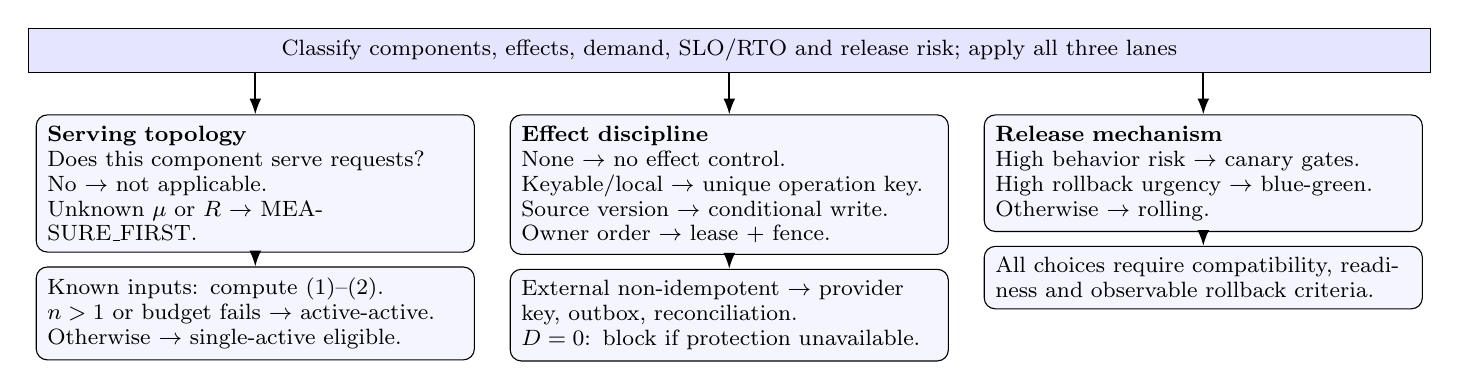
\begin{tikzpicture}[font=\fontsize{8}{9}\selectfont, >=Latex,
 box/.style={draw,rounded corners,align=left,inner sep=4pt,text width=2.08in,fill=blue!4},
 line/.style={->,semithick}]
\node[draw,fill=blue!10,align=center,text width=6.9in,inner sep=4pt] (input) at (0,0)
 {Classify components, effects, demand, SLO/RTO and release risk; apply all three lanes};
\node[box,anchor=north] (a) at (-2.37in,-.32in) {\textbf{Serving topology}\\Does this component serve requests?\\No $\to$ not applicable.\\Unknown $\mu$ or $R$ $\to$ MEASURE\_FIRST.};
\node[box,anchor=north] (b) at (0,-.32in) {\textbf{Effect discipline}\\None $\to$ no effect control.\\Keyable/local $\to$ unique operation key.\\Source version $\to$ conditional write.\\Owner order $\to$ lease + fence.};
\node[box,anchor=north] (c) at (2.37in,-.32in) {\textbf{Release mechanism}\\High behavior risk $\to$ canary gates.\\High rollback urgency $\to$ blue-green.\\Otherwise $\to$ rolling.};
\node[box,below=5pt of a] (a2) {Known inputs: compute (1)--(2).\\$n>1$ or budget fails $\to$ active-active.\\Otherwise $\to$ single-active eligible.};
\node[box,below=5pt of b] (b2) {External non-idempotent $\to$ provider key, outbox, reconciliation.\\$D=0$: block if protection unavailable.};
\node[box,below=5pt of c] (c2) {All choices require compatibility, readiness and observable rollback criteria.};
\foreach \x in {a,b,c} \draw[line] (input.south -| \x.north)--(\x.north);
\draw[line] (a)--(a2);\draw[line] (b)--(b2);\draw[line] (c)--(c2);
\end{tikzpicture}

\caption{Three independent selection lanes. A checkout API can receive active-active serving, provider idempotency controls and a canary release simultaneously. The measurement exit applies only to request-serving components.}\label{fig:selection}
\end{figure*}

For illustration, $\lambda_{\rm peak}=600$, $\mu=120$ requests/s and $h=0.20$ give $\lceil600/96\rceil=7$. Six replicas provide 576 requests/s after reserve and fail the condition; seven provide 672 requests/s, or 72 requests/s beyond the assumed peak. These are declared inputs and arithmetic, not observations. The availability screen remains symbolic until $f$ and $R$ are measured. Table~\ref{tab:mapping} gives composite outcomes.

\begin{table}[t]\caption{Workload-to-pattern mapping}\label{tab:mapping}
\centering\footnotesize
\begin{tabularx}{\columnwidth}{p{.77in}YY}\toprule
Workload & Serving plan & Effect discipline\\\midrule
Checkout API & Sized active-active & Provider key; reconcile capture\\
Internal UI & (1)--(2) determine eligibility & Keyed local writes where needed\\
Ordered feed job & N/A & Source version check; lease + fence for owner-defined order or costly contention\\
Export API + job & Active-active API & Per-export key; bounded workers\\\bottomrule
\end{tabularx}
\end{table}

\section{Highlander Architecture and Safety}
\subsection{Effect boundary and atomic ownership}
Figure~\ref{fig:architecture} separates requests from asynchronous work. For order-confirmation email, an outbox durably records intent, while a provider key or reconciliation addresses an ambiguous acknowledgment. Payment capture needs provider idempotency. An inventory feed with usable source versions can use a conditional version write; a search-index alias whose order is determined by its current publisher needs epoch fencing. Loyalty accrual often admits a unique business operation key. A system with several sinks needs protection at each sink; one database transaction cannot confer exactly-once behavior on an uncooperative external API.

\begin{figure}[t]\centering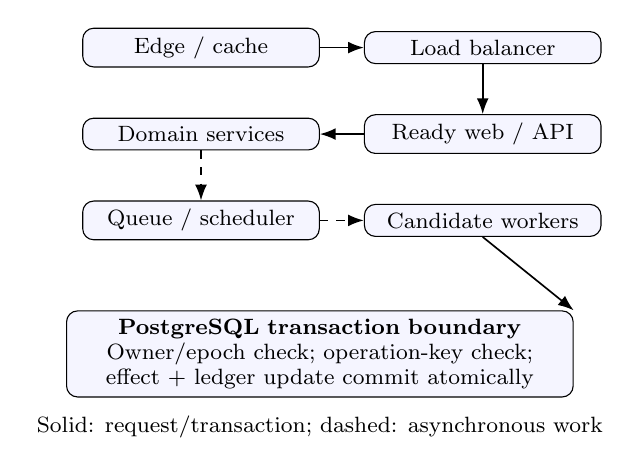
\begin{tikzpicture}[font=\fontsize{8}{9}\selectfont,>=Latex,
 n/.style={draw,rounded corners,align=center,inner sep=3pt,fill=blue!4},
 line/.style={->,semithick}]
\node[n,text width=1.1in] (edge) at (0,0) {Edge / cache};
\node[n,text width=1.1in,right=.22in of edge] (lb) {Load balancer};
\node[n,text width=1.1in,below=.25in of lb] (web) {Ready web / API};
\node[n,text width=1.1in,left=.22in of web] (domain) {Domain services};
\node[n,text width=1.1in,below=.25in of domain] (queue) {Queue / scheduler};
\node[n,text width=1.1in,right=.22in of queue] (workers) {Candidate workers};
\node[n,text width=2.45in,below=.35in of queue.south east,anchor=north] (tx)
 {\textbf{PostgreSQL transaction boundary}\\Owner/epoch check; operation-key check;\\effect + ledger update commit atomically};
\draw[line] (edge)--(lb);\draw[line] (lb)--(web);\draw[line] (web)--(domain);
\draw[line,dashed] (domain)--(queue);\draw[line,dashed] (queue)--(workers);
\draw[line] (workers.south)--(tx.north east);
\node[font=\fontsize{8}{9}\selectfont,below=3pt of tx] {Solid: request/transaction; dashed: asynchronous work};
\end{tikzpicture}

\caption{Reference architecture. The asynchronous branch is dashed. In the testbed, ownership validation, ledger insertion and effect mutation share a PostgreSQL transaction boundary.}\label{fig:architecture}
\end{figure}

Our PostgreSQL implementation binds ownership and epoch: an owner row $(k,holder,e,expires\_at)$ is changed by a conditional update on the database clock. Acquisition assigns holder, increasing epoch and expiry in the \emph{same} transaction. Renewal requires matching holder and epoch and an unexpired row. Each process incarnation has a UUID. A sink-fenced write locks that row and atomically checks authority with its ledger/state update.

We call this the \emph{lease-then-epoch race}: W1 acquires a Kubernetes Lease, pauses before requesting a separate epoch, and resumes after W2 has acquired a lease and token. Giving W1 a later token now legitimizes a zombie. Our protocol has no separate token-allocation operation: W1's delayed conditional acquisition is rejected while W2 owns an unexpired row. A pause after successful acquisition leaves W1 with its old epoch. Figure~\ref{fig:zombie}(b) illustrates this fix. A Kubernetes-only alternative must bind a holder change and epoch to the same compare-and-swap update, preserve monotonicity across object recreation, and use unique incarnation identities; it is not the protocol evaluated here.

\subsection{State transitions and safety property}
Table~\ref{tab:states} and Fig.~\ref{fig:states} describe local control states. ``Active'' is a client's belief, not proof that other processes stopped. Shutdown and uncertain renewal enter Draining. Crashes from Candidate, Active or Draining enter Failed; recovery returns to Standby only after durable-state reconciliation.

\begin{table}[t]\caption{Worker transitions}\label{tab:states}
\centering\footnotesize
\begin{tabularx}{\columnwidth}{p{.61in}YY}\toprule
From & Event [guard] / action & To\\\midrule
Standby & work [enabled] / acquire & Candidate\\
Candidate & grant [atomic CAS wins] / begin & Active\\
Candidate & denied [valid owner] / back off & Standby\\
Active & renew fails [uncertain] / stop admission & Draining\\
Active & shutdown [requested] / checkpoint & Draining\\
Draining & settled [durable checkpoint] / stop & Standby\\
Candidate, Active, Draining & crash [any] / no further action & Failed\\
Failed & recover [reconciled] / rejoin & Standby\\\bottomrule
\end{tabularx}
\end{table}

\begin{figure*}[t]\centering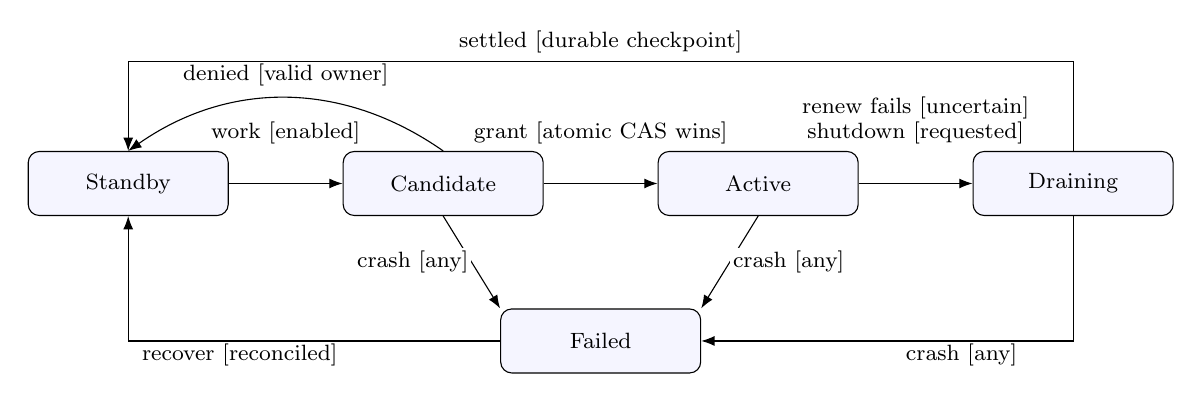
\begin{tikzpicture}[font=\fontsize{8}{9}\selectfont,>=Latex,
 s/.style={draw,rounded corners,minimum width=1in,minimum height=.32in,fill=blue!4},
 lab/.style={font=\fontsize{8}{9}\selectfont,align=center,fill=white,inner sep=1pt}]
\node[s] (s) at (0,0) {Standby};\node[s] (c) at (4,0) {Candidate};
\node[s] (a) at (8,0) {Active};\node[s] (d) at (12,0) {Draining};
\node[s] (f) at (6,-2) {Failed};
\draw[->] (s)--node[lab,above,yshift=13pt]{work [enabled]}(c);
\draw[->] (c)--node[lab,above,yshift=13pt]{grant [atomic CAS wins]}(a);
\draw[->] (c.north) to[out=145,in=35] node[lab,above,yshift=3pt]{denied [valid owner]}(s.north);
\draw[->] (a)--node[lab,above,yshift=13pt]{renew fails [uncertain]\\shutdown [requested]}(d);
\draw[->] (c.south)--node[lab,left]{crash [any]}(f.north west);
\draw[->] (a.south)--node[lab,right]{crash [any]}(f.north east);
\draw[->] (d.south) |- node[lab,pos=.65,below]{crash [any]}(f.east);
\draw[->] (f.west) -| node[lab,pos=.35,below]{recover [reconciled]}(s.south);
\draw[->] (d.north) -- (12,1.55) -- node[lab,above,yshift=2pt]{settled [durable checkpoint]} (0,1.55) -- (s.north);
\end{tikzpicture}

\caption{Local states with event [guard] labels. The curved denial edge returns Candidate to Standby.}\label{fig:states}
\end{figure*}

For the combined discipline, let $e_{\rm current}(k)$ be the durable current epoch and $\mathcal{K}(k)$ the committed operation keys. The participating sink enforces
\begin{equation}
\operatorname{accept}(k,e,op)\Rightarrow e\geq e_{\rm current}(k)\land op\notin \mathcal{K}(k).\label{eq:safety}
\end{equation}
In the co-located fenced conditions, the implementation strengthens the epoch check to equality with the current holder and valid expiry; tokens are never accepted merely because a client presents a larger number. The effect and ledger update commit atomically. Monotonic epoch issuance and a serialized check-and-write reject a former epoch after its successor is installed. Atomic uniqueness rejects an already committed operation key even within the same epoch. This proves neither cross-sink atomicity nor exactly-once external effects, and does not forbid an earlier valid write before the successor acquires ownership. In fence-only C2f, only the epoch clause is enforced; in unique-only C1u, only the operation-key clause is enforced. C1v instead checks a monotone data version at the sink without acquiring ownership.

\subsection{Time and failure assumptions}
A client-side safety deadline is $t_{\rm renew}+L-\delta$: effects must finish before that deadline. For Kubernetes Lease clients, expiry is judged from local observations, not an API-server expiry clock. Here $\delta$ conservatively includes clock-\emph{rate} drift between candidates, observation delay and write-to-commit time \cite{r24}. No finite client-only margin proves safety under unbounded pauses. In our PostgreSQL implementation the database clock decides expiry and the sink transaction decides authority; client stopping is an optimization, not its safety foundation.

Measured from the last successful renewal, acquisition and activation satisfy $R_{\rm renew}\leq L+P+S$ under bounded coordination and scheduling. From a crash $\Delta$ after renewal, time to the first accepted write instead satisfies
\begin{equation}
R_{\rm accept}\leq\max(0,L-\Delta)+P+S+W.\label{eq:takeover}
\end{equation}
$P$ covers detection/polling and coordinator response; $S$ covers activation and work preparation through the first successful submission; $W$ covers sink acceptance. A drain term $G$ is added only when a required serialized drain extends beyond expiry, not when it already occurred inside $L$. Unbounded partition or sink delay invalidates a finite bound. Expand/contract schema changes and backward-compatible checkpoints remain necessary: neither a traffic switch nor a ready Pod guarantees a safe worker-state rollback \cite{r19}.

\begin{figure*}[t]\centering
\begin{minipage}{.48\textwidth}\centering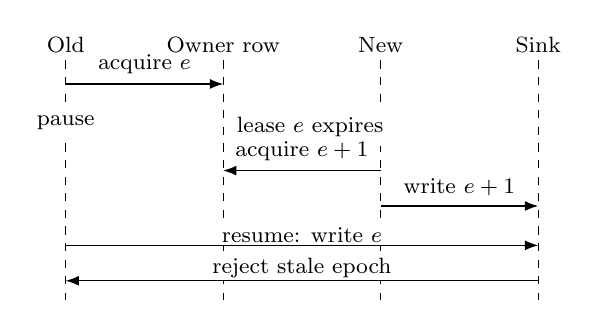
\begin{tikzpicture}[font=\fontsize{8}{9}\selectfont,>=Latex]
\foreach \x/\t in {0/Old,2/Owner row,4/New,6/Sink}{\node at (\x,0){\t};\draw[dashed] (\x,-.2)--(\x,-3.25);}
\draw[->] (0,-.5)--node[above]{acquire $e$}(2,-.5);
\node[fill=white] at (0,-1){pause};
\node[fill=white,anchor=west] at (2.05,-1.05){lease $e$ expires};
\draw[->] (4,-1.6)--node[above]{acquire $e+1$}(2,-1.6);
\draw[->] (4,-2.05)--node[above]{write $e+1$}(6,-2.05);
\draw[->] (0,-2.55)--node[above,fill=white,inner sep=1pt]{resume: write $e$}(6,-2.55);
\draw[->] (6,-3)--node[above,fill=white,inner sep=1pt]{reject stale epoch}(0,-3);
\end{tikzpicture}
\\(a) Stale effect after lease expiry\end{minipage}\hfill
\begin{minipage}{.48\textwidth}\centering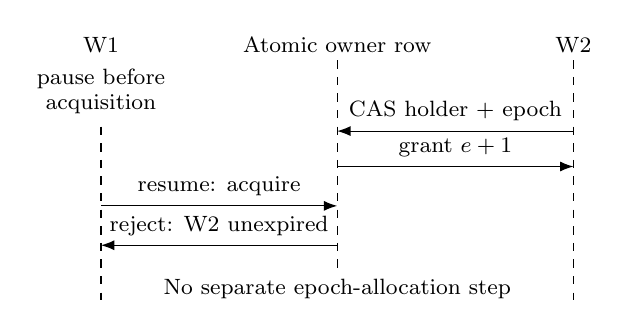
\begin{tikzpicture}[font=\fontsize{8}{9}\selectfont,>=Latex]
\foreach \x/\t in {0/W1,3/Atomic owner row,6/W2}{\node at (\x,0){\t};\draw[dashed] (\x,-.2)--(\x,-3.25);}
\node[fill=white,align=center] at (0,-.6){pause before\\acquisition};
\draw[->] (6,-1.1)--node[above]{CAS holder + epoch}(3,-1.1);
\draw[->] (3,-1.55)--node[above]{grant $e+1$}(6,-1.55);
\draw[->] (0,-2.05)--node[above]{resume: acquire}(3,-2.05);
\draw[->] (3,-2.55)--node[above]{reject: W2 unexpired}(0,-2.55);
\node[fill=white,align=center] at (3,-3.1){No separate epoch-allocation step};
\end{tikzpicture}
\\(b) Atomic acquisition rejects a delayed contender\end{minipage}
\caption{Two distinct pause hazards. (a) A sink rejects an old epoch after a successor's publication. (b) Binding holder and epoch in one conditional transaction prevents the separate-allocation race.}\label{fig:zombie}
\end{figure*}

\section{Evaluation}
\subsection{Testbed and scope}
The completed controlled experiment executes PostgreSQL 16.15 sink functions and SQL attempt logs on a GitHub Actions PostgreSQL service. The restricted remote sink uses a separate schema and role without access to ownership; this is a permission boundary in one database instance, not an independent networked service. A separate planned campaign uses a two-node kind cluster, three Python candidates and a CPU-limited HTTP service. The eight mechanism combinations are listed in Table~\ref{tab:ablation}.

\begin{table}[t]\caption{Mechanism ablations. Lease is a PostgreSQL owner-row lease; co-located fence checks holder, epoch and expiry; C3r checks its sink epoch.}\label{tab:ablation}
\centering\footnotesize
\setlength{\tabcolsep}{2.5pt}
\begin{tabular}{lccccc}\toprule
Condition & Lease & Fence & Version & Unique & Replay\\\midrule
C1 & -- & -- & -- & -- & --\\
C1u & -- & -- & -- & Yes & --\\
C1v & -- & -- & Yes & -- & --\\
C2 & Yes & -- & -- & -- & --\\
C2f & Yes & Yes & -- & -- & --\\
C3 & Yes & Yes & -- & Yes & --\\
C3r & Yes & Remote & -- & Yes & --\\
C4 & Yes & Yes & -- & Yes & Yes\\\bottomrule
\end{tabular}
\end{table}

\subsection{Methodology and hypotheses}
The planned kind campaign would compare the eight mechanisms at $b=10$ and $d=1$ s with 30 trials per applicable workload and 1,000 items per trial; a separate sweep varies $b\in\{1,10,100\}$ and $d\in\{0,1,5\}$ s. The duplicate workload reuses operation keys. In the ordered workload, the source assigns comparable versions independently of any lease; each publication uses a distinct operation key. A version regression is an accepted lower source version, and an epoch regression is an accepted lower authority epoch. Both use recorded pre-write state. Epoch regression applies only where a lease epoch exists.

In the planned fault campaign, a worker prepares a batch, self-stops with SIGSTOP, and resumes with SIGCONT after a successor grant or first write. The runner verifies process state and a stopped heartbeat \cite{r25}; batch size controls exposure. Hypotheses distinguish repeated-key suppression (C1u/C3), source-version monotonicity (C1v), authority fencing (C2 versus C2f/C3), and stable replay (C4). C3r advances its feed-wide remote fence on the successor's first remote write, leaving a grant-to-write window. This sink boundary explains why a prior-epoch accept can occur even when no version regression occurs.

The completed lost-ack series retries a current-owner operation key after 50 ms under a predeclared 5\% acknowledgment-loss input. C2f may repeat the effect, C3 rejects an ambiguous repeat, and C4 replays its cached response. The planned cluster campaign would separately report rejected attempts, preparation CPU, invalid trials and released at-risk submissions. For zero observed safety violations, it would use a one-sided 95\% Clopper--Pearson upper bound; continuous trial summaries would use 10,000 percentile-bootstrap resamples with seed 2026. These inferential procedures are not applied to the scripted data.

Planned takeover trials vary $L\in\{5,10,15,30\}$ s with SIGKILL and no lease release, bracket the kill, and compare first accepted writes with (4). Serving tests would calibrate $\mu$ at a p99 objective, compare $n_{\rm req}-1$ with $n_{\rm req}$, and measure release intervals for rolling, blue-green and client-weighted canary. Replica-seconds proxy allocation rather than dollars; Table~\ref{tab:metrics} defines the endpoints.

\begin{table}[t]\caption{Evaluation endpoints}\label{tab:metrics}
\centering\footnotesize
\begin{tabularx}{\columnwidth}{p{.80in}YY}\toprule
Metric & Definition & Raw source\\\midrule
Duplicates & Accepted repeated key & Sink attempts\\
Version regressions & Accepted source version $<$ stored version; all conditions & Prior sink state\\
Epoch regressions & Accepted epoch $<$ maximum applied epoch; lease conditions & Prior sink state\\
Late accepts & Old epoch after grant, before new sink write & Grant/accept logs\\
Wasted work & Rejections; preparation CPU & Sink attempts\\
Takeover & Kill bracket to first effect & Fault/accept logs\\
p99; violations & Latency; SLO failures & HTTP requests\\
Release cost & Extra replica-seconds & Readiness logs\\\bottomrule
\end{tabularx}
\end{table}

\subsection{Results}
\begin{table*}[!t]\caption{Scripted SQLite interleaving outcomes. Counts reflect the specified schedule and sink rules, not failure-rate estimates.}\label{tab:results}
\centering\footnotesize\setlength{\tabcolsep}{6pt}
\begin{tabular}{lccccccc}\toprule
Condition & $n_D$ & $n_O$ & Duplicates & Version reg. & Epoch reg. & Late & Rejected$_O$\\\midrule
C1 & 1 & 30 & 100 & 2,071 & N/A & N/A & 0\\
C1u & 1 & 30 & 0 & 2,071 & N/A & N/A & 0\\
C1v & N/A & 30 & N/A & 0 & N/A & N/A & 2,071\\
C2 & 1 & 30 & 100 & 2,071 & 2,991 & N/A & 0\\
C2f & 1 & 30 & 0 & 0 & 0 & N/A & 3,000\\
C3 & 1 & 30 & 0 & 0 & 0 & 0 & 3,000\\
C3r & 1 & 30 & 0 & 0 & 0 & 9 & 2,991\\
C4 & 1 & 30 & 0 & 0 & 0 & N/A & 3,000\\\bottomrule
\end{tabular}
\par\vspace{4pt}\parbox{.95\textwidth}{\scriptsize $n_D/n_O$: scheduled duplicate/ordered runs; each run has 100 keys. Version and epoch regressions are separate outcomes on the ordered workload. Late means an accepted former-epoch write after grant and before the successor's first remote write. Rejected$_O$: delayed ordered attempts rejected by a guard. N/A: inapplicable or not measured. CPU and provider cost are not measured.}
\end{table*}

\subsubsection{Scheduled PostgreSQL interleavings}
The completed study executes the PostgreSQL owner-row, sink, and remote-sink SQL functions under a controlled event schedule; the earlier SQLite rule-model study provides a comparison, not the primary result. Every ordered trial starts with a v1 publication on each key. Across \ObsOrderedRuns{} paired schedules of \ObsKeys{} keys per condition, the successor publishes v3 first for each shuffled key with a declared input probability of \ObsFirstProbabilityPct\%; the delayed former worker attempts v2. All conditions use the same trial seeds. A v2 accepted after v3 is a version regression, whereas an older epoch accepted after any successor write is an authority regression. These measures have different denominators and must not be conflated. In particular, the feed-wide authority metric may flag an old-epoch write even if that particular item has not received v3.

Table~\ref{tab:results} is generated from the PostgreSQL trial CSV. The unguarded C1 and C2 conditions each admit \ObsOrderedCOneVersion{} version regressions. C2 also admits \ObsOrderedCTwoEpoch{} epoch regressions. C1v rejects late lower-version attempts without acquiring a lease. The co-located fence rejects all delayed former-epoch attempts after grant, so C2f, C3, and C4 have zero observed epoch regressions under this schedule. These are observed SQL outcomes in the specified trial cells; no independence-based failure-rate bound follows from repeated keys or chosen ordering.

C3r stores one remote sink epoch for the whole feed, advancing it on the successor's first remote effect. Its \ObsOrderedRemoteLate{} accepted former-epoch effects occur after the successor grant and before that first remote write. The old effects precede v3 on their individual keys, explaining why this cell has zero version regressions despite a grant-to-write authority gap. In the after-grant sweep, the successor first remote write is scheduled at \ObsFirstWriteS{} s and the former batch resumes at $d\in\{0,1,5\}$ s. Each cell is a single deterministic schedule of \ObsKeys{} keys. The remote sink accepts all \ObsAfterRemoteBefore{} older-epoch attempts at $d=0$ and $d=1$ s and rejects all at $d=5$ s; the co-located fence rejects all former-epoch attempts at each delay. Figure~\ref{fig:sweep} plots only the tested delays; intermediate delays were not measured.

The duplicate pause series has \ObsDuplicateRuns{} run per applicable condition and repeats the same business operation keys after takeover. C1 and C2 accept those duplicate effects; C1u enforces uniqueness. The co-located fence rejects delayed repeats in C2f/C3/C4, while C3r uses its unique key and/or remote epoch. This single run does not estimate a population duplicate rate. The independent lost-ack series exercises retries by the \emph{current} owner: \ObsReplayRuns{} paired schedules use \ObsKeys{} initial calls each, \ObsLostPct\% input acknowledgment-loss probability, and \ObsRetryMs{} ms before retry. Of \ObsReplayRetries{} realized retries per condition, C2f accepts duplicate effects, C3 rejects duplicates without resolving the caller's response, and C4 returns stable cached responses with zero observed mismatches (Table~\ref{tab:replay}).
\begin{table}[t]\caption{Scripted lost-ack retries by the current owner. Outcome counts follow the chosen loss draws; zero response mismatches were observed.}\label{tab:replay}
\centering\footnotesize\setlength{\tabcolsep}{3.5pt}
\begin{tabular}{lrrrr}\toprule
Condition & Retry calls & Dup. accepted & Ambig. rejected & Stable replay\\\midrule
C2f & 165 & 165 & 0 & 0\\
C3 & 165 & 0 & 165 & 0\\
C4 & 165 & 0 & 0 & 165\\\bottomrule
\end{tabular}
\end{table}

\begin{figure}[t]\centering
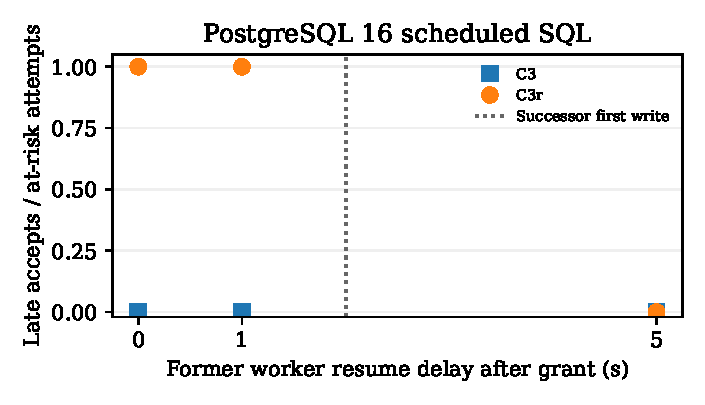
\includegraphics[width=.98\columnwidth]{figures/after_grant.pdf}
\caption{PostgreSQL after-grant late-accept fraction from scheduled SQL trial rows. Markers are tested delays; the dotted line is the scheduled first successor write, not an observed latency.}\label{fig:sweep}
\end{figure}

\subsubsection{Active handover and acquisition races}
The former writer starts submitting before takeover, while a separate thread expires the setup lease, acquires epoch~\ObsExpiredEpoch{} and begins successor writes. Each of \ObsThreadRepeats{} repetitions includes \ObsThreadRuns{} runs per condition with \ObsThreadKeys{} keys; randomized microdelays and host scheduling vary the overlap. The former's setup lease is expired by an administrative update after its initial batch commits, and the successor then acquires epoch~\ObsExpiredEpoch{} through \texttt{own.acquire}. Table~\ref{tab:concurrency} counts legitimate pre-grant accepts separately from former writes committed after grant; the latter are obtained from the SQL \texttt{late\_accepts} view. The co-located fences have no post-grant former accepts; C3r has \ObsThreadRemoteTotal{} across the five repetitions, ranging from \ObsThreadRemoteMin{} to \ObsThreadRemoteMax{} per repetition. Separate two-session races on \ObsFreshWins{} fresh keys each produce one winner at epoch~\ObsFreshEpoch{}; \ObsExpiredWins{} expired-key takeover races each produce one winner at epoch~\ObsExpiredEpoch{}, incrementing the prior epoch by \ObsAcquisitionDelta{}. These finite races test one PostgreSQL instance, not independent network partitions.
\begin{table}[t]\caption{Active-handover races on PostgreSQL. Only SQL commits after epoch-2 grant count as late accepts.}\label{tab:concurrency}
\centering\footnotesize\setlength{\tabcolsep}{3.5pt}
\begin{tabular}{lrrr}\toprule
Condition & Runs & Pre-grant accepted & Late / post-grant\\\midrule
C2f & 150 & 1,494 & 0/4,138\\
C3 & 150 & 1,487 & 0/4,131\\
C4 & 150 & 1,490 & 0/4,125\\
C3r & 150 & 1,866 & 436/4,134\\\bottomrule
\end{tabular}
\end{table}


The PostgreSQL 16.15 CI run reports \ObsRawRuns{} raw schedules, 43 summary rows, zero mismatched cell metrics relative to the SQLite model, and 53 passing tests (run 36291161498). The equality of selected aggregates validates agreement under shared scripted inputs; it does not demonstrate independent production replication or cluster behavior. Neither deployment velocity, preparation CPU, replica-seconds, takeover latency, p99 latency, nor provider effects were measured, so no economic or downtime reduction is inferred.

\subsection{Threats to validity and artifact availability}
The planned kind cluster shares one host; CPU contention and host faults would correlate otherwise separate Pods. The scheduled study cannot characterize unconstrained concurrency; the threaded check covers limited real concurrency on one PostgreSQL instance. Neither measures cluster faults, external service behavior, or operational cost. Its restricted remote sink is a separate schema and role within the same PostgreSQL instance, with no network partition. Synthetic effects omit provider behavior, cache skew and session affinity. SIGSTOP captures a defined delayed batch rather than every possible partition. PostgreSQL's transaction boundary is stronger than many external sinks. Cluster clock changes can affect expiry; bound interpretation requires clock and delay assumptions as well as a point estimate.

\textit{Artifact Availability:} The paper, raw CSVs, SQL, and generators are archived at \url{https://github.com/nallabothukoteswar-wq/highlander-harness}, tag \texttt{paper-v9.1}; the earlier \texttt{paper-v9} snapshot is retained. The v9.1 handover generator was introduced at commit \texttt{a85c5ffaafa31bdb1c001b747c9ac837964a0440}. The measured handover run is archived at \url{https://github.com/nallabothukoteswar-wq/highlander-harness/actions/runs/36334206522}. The kind campaign runner remains under development; reported counts come from the included CSVs and scripts. No archival DOI is available.

\section{Discussion and Limitations}
Idempotency keys solve repeatable, keyable effects. A conditional version check blocks version regressions when source versions are comparable. Epoch fencing blocks epoch authority regressions for lease conditions when a lower epoch follows a higher one; a remote epoch fence can still admit an older epoch after a successor grant but before its first remote write. These metrics must be analyzed separately. Ownership can reduce contention and wasted work but does not prove that only one process is executing. An ordered workload must also define order within one epoch; our test worker publishes sequentially. If current-epoch operations can be reordered in transit, an additional version check is required. A fencing result must not be generalized to ordering that the sink never checks.

A payment or email provider remains outside the local transaction: an outbox preserves intent but cannot settle an unknown external outcome alone. Per-key ownership avoids a global bottleneck for independent feeds. Interactive APIs retain active-active capacity sizing even when their effect paths are serialized. A low-traffic internal interface is single-active only when capacity and availability constraints both pass. During coordinator loss, stopping effects favors safety at the cost of progress. Blue-green rollback needs compatible state; canaries need representative traffic and version-tagged metrics. PodDisruptionBudgets restrict voluntary disruptions, not node loss \cite{r23}.

The analytical results establish a decision decomposition and a conditional sink safety argument. The scheduled PostgreSQL outcomes expose distinct version, epoch, and remote late-accept cases under their chosen schedules; they do not establish production speedup, cost savings, or failure-rate reduction. PostgreSQL protocol tests for uniqueness, fencing, atomic acquisition, response replay and restricted remote-sink access passed in the cited CI run; the scheduled study does not exercise a Kubernetes failover campaign.

\section{Conclusion and Future Work}
Workload-aware deployment requires separate decisions for serving topology, effect discipline and release mechanism. Atomic ownership binds a holder to its fencing epoch, while atomic operation-key handling prevents repeat effects. The distinction is necessary to evaluate Highlander as a single-effective-writer policy without attributing uniqueness guarantees to leadership. Future work should assess production traces, multi-zone coordinator faults, reordered current-epoch publications and real provider idempotency contracts. The reported sink observations cover scheduled SQL writes and bounded single-instance thread races; cluster and production claims require the planned kind campaign.

\begin{thebibliography}{25}
\raggedright
\setlength{\itemsep}{-1pt}
\bibitem{r1} Kubernetes Authors, ``Deployments,'' \emph{Kubernetes Documentation}.
{[}Online{]}. Available:
\url{https://kubernetes.io/docs/concepts/workloads/controllers/deployment/}
(accessed Sep.~26, 2026).
\bibitem{r2} M. Fowler, ``Blue Green Deployment,'' 2010. {[}Online{]}. Available:
\url{https://martinfowler.com/bliki/BlueGreenDeployment.html} (accessed
Sep.~26, 2026).
\bibitem{r3} M. Fowler, ``Canary Release,'' 2014. {[}Online{]}. Available:
\url{https://martinfowler.com/bliki/CanaryRelease.html} (accessed Sep.~26,
2026).
\bibitem{r4} C. G. Gray and D. R. Cheriton, ``Leases: An Efficient Fault-Tolerant
Mechanism for Distributed File Cache Consistency,'' in \emph{Proc. ACM
SOSP}, 1989. \url{https://doi.org/10.1145/74850.74870}
\bibitem{r5} M. Burrows, ``The Chubby Lock Service for Loosely-Coupled Distributed
Systems,'' in \emph{Proc. USENIX OSDI}, 2006.
\url{https://www.usenix.org/conference/osdi-06/chubby-lock-service-loosely-coupled-distributed-systems}
\bibitem{r6} P. Hunt, M. Konar, F. P. Junqueira, and B. Reed, ``ZooKeeper: Wait-free
Coordination for Internet-scale Systems,'' in \emph{Proc. USENIX ATC},
2010.
\url{https://www.usenix.org/conference/usenix-atc-10/zookeeper-wait-free-coordination-internet-scale-systems}
\bibitem{r7} D. Ongaro and J. Ousterhout, ``In Search of an Understandable Consensus
Algorithm,'' in \emph{Proc. USENIX ATC}, 2014.
\url{https://www.usenix.org/conference/atc14/technical-sessions/presentation/ongaro}
\bibitem{r8} M. Kleppmann, \emph{Designing Data-Intensive Applications}. O'Reilly
Media, 2017. \url{https://dataintensive.net/}
\bibitem{r9} P. Helland, ``Idempotence Is Not a Medical Condition,'' \emph{ACM
Queue}, 2012. \url{https://queue.acm.org/detail.cfm?id=2187821}
\bibitem{r10} H. Garcia-Molina and K. Salem, ``Sagas,'' in \emph{Proc. ACM SIGMOD},
1987. \url{https://doi.org/10.1145/38713.38742}
\bibitem{r11} A. Verma \emph{et al.}, ``Large-scale cluster management at Google with
Borg,'' in \emph{Proc. ACM EuroSys}, 2015.
\url{https://research.google/pubs/large-scale-cluster-management-at-google-with-borg/}
\bibitem{r12} M. Schwarzkopf, A. Konwinski, M. Abd-El-Malek, and J. Wilkes, ``Omega:
flexible, scalable schedulers for large compute clusters,'' in
\emph{Proc. ACM EuroSys}, 2013.
\url{https://research.google/pubs/omega-flexible-scalable-schedulers-for-large-compute-clusters/}
\bibitem{r13} M. Tirmazi \emph{et al.}, ``Borg: the Next Generation,'' in \emph{Proc.
ACM EuroSys}, 2020.
\url{https://doi.org/10.1145/3342195.3387517}
\bibitem{r14} T. Akidau \emph{et al.}, ``MillWheel: Fault-Tolerant Stream Processing
at Internet Scale,'' \emph{Proc. VLDB Endowment}, 2013.
\url{https://research.google/pubs/millwheel-fault-tolerant-stream-processing-at-internet-scale/}
\bibitem{r15} R. Ananthanarayanan \emph{et al.}, ``Photon: Fault-tolerant and Scalable
Joining of Continuous Data Streams,'' in \emph{Proc. ACM SIGMOD}, 2013.
\url{https://research.google/pubs/photon-fault-tolerant-and-scalable-joining-of-continuous-data-streams/}
\bibitem{r16} G. Schermann, J. Cito, P. Leitner, U. Zdun, and C. H. Gall, ``We're
doing it live: A multi-method empirical study on continuous
experimentation,'' \emph{Information and Software Technology}, vol.~99,
2018. \url{https://eprints.cs.univie.ac.at/5953/}
\bibitem{r17} Š. Davidovič and B. Beyer, ``Canary Analysis Service,'' \emph{ACM
Queue}, vol.~16, no. 1, 2018.
\url{https://queue.acm.org/detail.cfm?id=3194655}
\bibitem{r18} Kubernetes Authors, ``Jobs,'' \emph{Kubernetes Documentation}.
{[}Online{]}. Available:
\url{https://kubernetes.io/docs/concepts/workloads/controllers/job/} (accessed
Sep.~26, 2026).
\bibitem{r19} Kubernetes Authors, ``Liveness, Readiness, and Startup Probes,''
\emph{Kubernetes Documentation}. {[}Online{]}. Available:
\url{https://kubernetes.io/docs/concepts/workloads/pods/probes/} (accessed
Sep.~26, 2026).
\bibitem{r20} Kubernetes Authors, ``Leases,'' \emph{Kubernetes Documentation}.
{[}Online{]}. Available:
\url{https://kubernetes.io/docs/concepts/architecture/leases/} (accessed
Sep.~26, 2026).
\bibitem{r21} Kubernetes Authors, ``Horizontal Pod Autoscaling,'' \emph{Kubernetes
Documentation}. {[}Online{]}. Available:
\url{https://kubernetes.io/docs/concepts/workloads/autoscaling/horizontal-pod-autoscale/}
(accessed Sep.~26, 2026).
\bibitem{r22} Argo Project, ``Canary Deployment Strategy,'' \emph{Argo Rollouts
Documentation}. {[}Online{]}. Available:
\url{https://argo-rollouts.readthedocs.io/en/stable/features/canary/}
(accessed Sep.~26, 2026).
\bibitem{r24} Kubernetes Authors, ``leaderelection package,'' client-go source documentation. [Online]. Available: \url{https://pkg.go.dev/k8s.io/client-go/tools/leaderelection} (accessed Sep. 26, 2026).
\bibitem{r25} Linux man-pages project, ``pid\_namespaces(7),'' \emph{Linux manual page}. [Online]. Available: \url{https://man7.org/linux/man-pages/man7/pid_namespaces.7.html} (accessed Sep. 26, 2026).
\bibitem{r23} Kubernetes Authors, ``Specifying a Disruption Budget for your
Application,'' \emph{Kubernetes Documentation}. {[}Online{]}. Available:
\url{https://kubernetes.io/docs/tasks/run-application/configure-pdb/}
(accessed Sep.~26, 2026).
\end{thebibliography}
\end{document}
